\chapter{Introduction}
\justify

The Open-source Intelligence Data Mining System (OSINT), as depicted in Figure 1.1, is an advanced software specifically designed to assist law enforcement agencies, such as the police department, in crime investigations by effectively analyzing call data records (CDRs) and tower dump data. It offers a comprehensive range of features crucial for conducting successful criminal investigations.

\begin{figure}
    \centering
    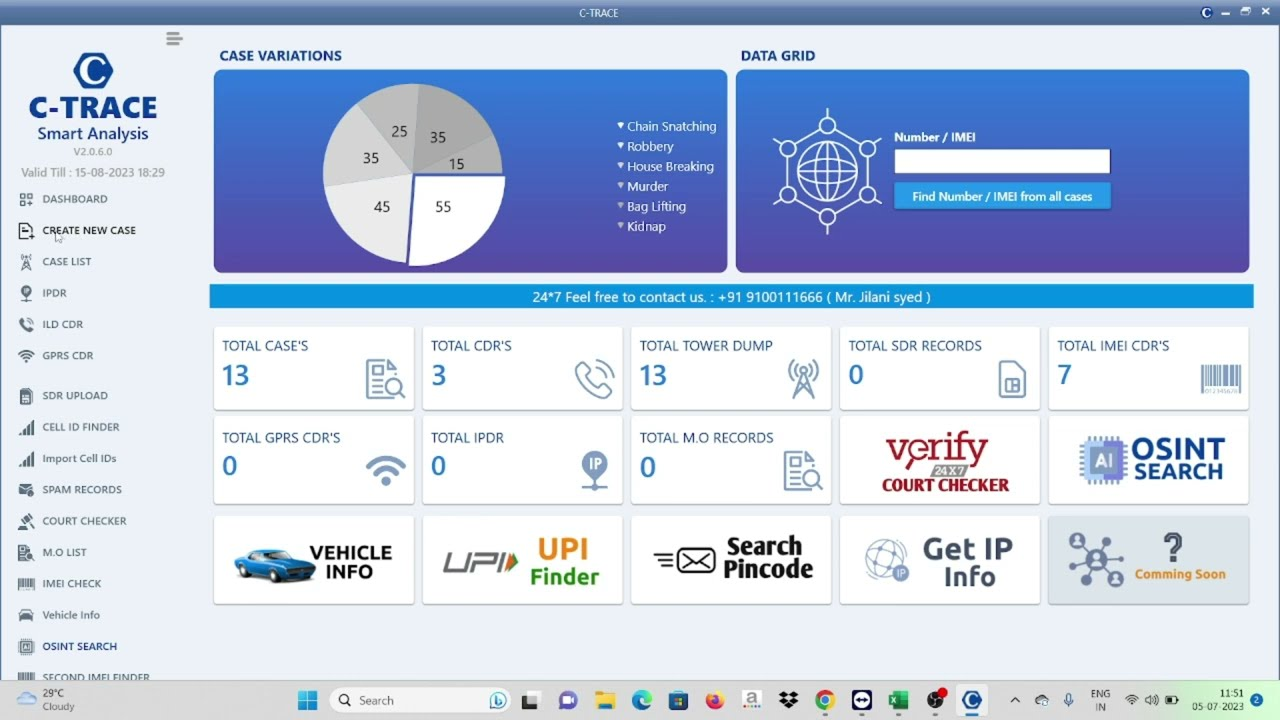
\includegraphics[width=1\linewidth]{Media/maxresdefault.jpg}
    \caption{C-Trace OSINT Software}
    \label{fig:CTraceOSINTSoftware}
\end{figure}

The primary objective of this application is to provide law enforcement agencies with a rapid and efficient means of analyzing call data records (CDRs) and tower dump data. C-Trace OSINT software acts as a force multiplier, empowering investigators to make informed decisions and progress their investigations more effectively.

\section{What is OSINT Data Mining System ?}

The developed application is specifically designed for use by police departments only in solving crime cases by analyzing call data records (CDRs) and tower dump data. This software provides a detailed report on individuals using their phone number, IMEI number, PAN number, etc. It can extract tower data to identify all phone users within a specific tower, using azimuth ID. The report includes information such as the person's vehicle details, location data, IMEI numbers, phone numbers, PAN numbers, MNP details, IP information, and more. The software generates a PDF report that encompasses all relevant information about the individual.

\section{Features of OSINT Software}

The developed software provides a range of powerful search functionalities based query. Below are some of the key features offered:

\begin{enumerate}[label=\textbf{\roman*.}]
    \item \textbf{Vehicle information} : RC MH02ZX1234
    \item \textbf{IP Lookup} : IP 192.168.01.01
    \item \textbf{Pin code search} : PIN 524455
    \item \textbf{IMEI Search} : IMEI 45671234765823 \\
        You can Get Device Model details
    \item \textbf{PNR Search} : PNR 456789101 \\
        Check your train ticket status. Access passenger, seat, boarding, and destination info.
    \item \textbf{IFSC Search} : (e.g., "IFSC SBIN0062517" or "IFSC SBI ATTAPUR") \\
        Find bank details and IFSC codes for banks and cities.
    \item \textbf{UPI Search} : UPI 8465802838 \\
        Now, you can effortlessly retrieve UPI ID details by simply sending a UPI Mobile number. For instance, send UPI 8465802838
    \item \textbf{Court Case Search} : CC Name \\
        Now you can effortlessly track court cases of old offenders and suspects with our new Court Case Search feature. Simply send "CC Name" followed by the name of the individual, just like this: CC Prakash.
    \item \textbf{OSINT Search} : OSINT 9848012345 \\
        You can access names linked to phone numbers, UPI IDs, photos, social media accounts, and more.
    \item \textbf{Phone Number to Gas Connection search} : GAS 9848012345
    \item \textbf{Cell ID Search} : BTS 4044349032727 \\
        You can tower ID address and azimuth direction in Google Maps
    \item \textbf{MNP Lookup} : Network 9848012345 \\
        You can get mobile number portability details and Operator details
    \item \textbf{IMEI Last digit finder} : FULL IMEI 45231671101234 \\
        You can identify the last digit of an IMEI number.
\end{enumerate}

\section{Plugins Integrated with C-Trace OSINT Software}

This software is integrated with additional tools such as Verify 24x7 Court Checker, OSINT
Search, and Vehicle Information. These plugins enhance the software's capabilities and provide additional functionalities to law enforcement agencies.

\subsection{Verify 24x7 Court checker}

The Verify 24x7 Court checker is a third party tool that has large collection of court cases in India containing millions of records and updated on a daily basis. Given a name and address, our smart, proprietary algorithms retrieve matching cases in a few seconds.

This plugin allows users to verify the court case status of an individual by entering their name. This feature provides information on the individual's court cases, including the case number, court name, and case status. By utilizing this feature, law enforcement agencies can quickly verify the court status of suspects and offenders, aiding in their investigations and intelligence gathering.

\subsection{OSINT Search}

OSINT Search is a feature that allows users to gather publicly available information about individuals, including personal and public details, to aid in investigations. By utilizing OSINT (Open-Source Intelligence) techniques, this feature helps retrieve relevant information about the suspect, such as their personal background, social
media activity, online presence, and other publicly accessible data. This
comprehensive search capability assists law enforcement agencies and investigators in building a more complete profile of the culprit, aiding in the investigation process.

\subsection{Vehicle Information}

Vehicle Information is a feature that allows users to obtain details about a specific vehicle using its registration number. By inputting the vehicle number into the system, investigators can retrieve information such as the make, model, year of manufacture, color, and ownership details of the vehicle associated with that registration number. This feature is valuable in investigations as it helps identify and track vehicles linked to criminal activities, providing important leads for law enforcement agencies and helping them in their pursuit of the culprits.

\section*{The rest of the Report is organized as follows:}
\begin{itemize}
    \item \textbf{Chapter 2:} Tools and Technologies
    \item \textbf{Chapter 3:} Proposed Systems
    \item \textbf{Chapter 4:} Design
    \item \textbf{Chapter 5:} Implementation
    \item \textbf{Chapter 6:} Testing and Experimental Results
    \item \textbf{Chapter 7:} Conclusion and Future Scope
\end{itemize}

\newpage


